%\nocite{24253327}
%\nocite{0d7b89ad}
%\nocite{c2d89e8a}
%\nocite{de09a3f9}
\nocite{bc53e62a}
%\nocite{00000011}
In this subsubsection we categorify monoids with the method described earlier in this subsection to get the notion of monoidal category. Subsequently, it turns out that that we can define functors and natural transformations preserving the monoidal structure. We then do the same when the monoid is commutative. After this we look at an example regarding vector spaces before generalizing category theory to enriched category theory. From all this it will become quite clear that we can internalize monoids in monoidal categories and this will be utilized to define monads as oidification of monoid objects in monoidal categories. The original case of monads is the case $\mathbf{Cat}$. An even more special case is the restriction to a certain category of set-valued functors we allude to and provide references for. The monoidal objects there are operads\footnote{a word built from operation an monad} which were developed by May (among others) to study iterated loop spaces which can be used to define the homotopy groups and are hence of interest regarding the coherence conditions for higher categories
\\
But be warned that the discussion in this subsubsection is mostly superficial and we mostly provide only terminology. Unfortunately, we do not have the time (and means) here to prove any deep theorems like coherence theorems or the strictification theorem. We only provide the bare necessities needed to delve into the literaure we refer to.
\\\\
But now back to the salt mines. A set $\mathcal{M}_{\mathbf{C}}$ is a \textbf{monoidal category} if it is a $6$-tuple
\begin{align*}
  \left(
    \mathbf{C},
    \otimes,
    \mathsf{A},
    1,
    \mathsf{L},
    \mathsf{R}
  \right)
\end{align*}
consisting of
\begin{enumerate}
\item[(1)]
a category $\mathbf{C}$
\item[(2)]
a functor
\begin{align*}
  \cdot
  \otimes
  \cdot
  \doteq
  \otimes
  \colon
  \mathbf{C}
  \times
  \mathbf{C}
  &\rightarrow
  \mathbf{C}
\end{align*}
\item[(3)]
for the functors
\begin{align*}
  \left(
    \cdot
    \otimes
    \cdot
  \right)
  \otimes
  \cdot
  \doteq
  {}_{\otimes}\otimes
  \colon
  \mathbf{C}
  \times
  \mathbf{C}
  \times
  \mathbf{C}
  &\rightarrow
  \mathbf{C}
  \\
  (X_{1},X_{2},X_{3})
  &\mapsto
  \otimes(\otimes(X_{1},X_{2}),X_{3})
  \\
  (f_{12},f_{34},f_{56})
  &\mapsto
  \otimes(\otimes(f_{12},f_{34}),f_{56})
  \\\\
  \cdot
  \otimes
  \left(
    \cdot
    \otimes
    \cdot
  \right)
  \doteq
  \otimes_{\otimes}
  \colon
  \mathbf{C}
  \times
  \mathbf{C}
  \times
  \mathbf{C}
  &\rightarrow
  \mathbf{C}
  \\
  (X_{1},X_{2},X_{3})
  &\mapsto
  \otimes(X_{1},\otimes(X_{2},X_{3}))
  \\
  (f_{12},f_{34},f_{56})
  &\mapsto
  \otimes(f_{12},\otimes(f_{34},f_{56}))
\end{align*}
a natural isomorphism
\begin{align*}
  \mathsf{A}
  \colon
  {}_{\otimes}\otimes
  &\Rightarrow
  \otimes_{\otimes}
\end{align*}
\item[(4)]
an object\footnote{don't mix this up with terminal objects since it is just an unfortunate notational coincidence as so often is the case for this symbol} $1$ of $\mathrm{ob}_{\mathbf{C}}$
\item[(5)]
for the functor
\begin{align*}
  \otimes(1,\cdot)
  \colon
  \mathbf{C}
  &\rightarrow
  \mathbf{C}
  \\
  X
  &\mapsto
  \otimes(1,X)
  \\
  f_{12}
  &\mapsto
  \otimes(\mathrm{id}_{1},f_{12})
\end{align*}
a natural isomorphism
\begin{align*}
  \mathsf{L}
  \otimes(1,\cdot)
  \colon
  &\Rightarrow
  \mathrm{id}_{\mathbf{C}}
\end{align*}
\item[(6)]
for the functor
\begin{align*}
  \otimes(\cdot,1)
  \colon
  \mathbf{C}
  &\rightarrow
  \mathbf{C}
  \\
  X
  &\mapsto
  \otimes(X,1)
  \\
  f_{12}
  &\mapsto
  \otimes(f_{12},\mathrm{id}_{1})
\end{align*}
a natural isomorphism
\begin{align*}
  \mathsf{R}
  \colon
  \otimes(\cdot,1)
  &\Rightarrow
  \mathrm{id}_{\mathbf{C}}
\end{align*}
\end{enumerate}
such that
\begin{enumerate}
\item[(MC1)]
the diagram
\[
\begin{tikzcd}[row sep=3.5em,column sep=0.4em]
  &
  (X_{1} \otimes X_{2})
  \otimes
  (X_{3} \otimes X_{4})
  \arrow{dr}{\mathsf{A}(X_{1},X_{2},X_{3} \otimes X_{4})}
  &
  \\
  \left(
    (X_{1} \otimes X_{2})
    \otimes
    X_{3}
  \right)
  \otimes
  X_{4}
  \arrow{ur}{\mathsf{A}(X_{1} \otimes X_{2},X_{3},X_{4})}
  \arrow[swap]{d}{\mathsf{A}(X_{1},X_{2},X_{3}) \otimes \mathrm{id}_{X_{4}}}
  &
  &
  X_{1}
  \otimes
  \left(
    X_{2}
    \otimes
    (X_{3} \otimes X_{4})
  \right)
  \\
  \left(
    X_{1}
    \otimes
    (X_{2} \otimes X_{3})
  \right)
  \otimes
  X_{4}
  \arrow{rr}{\mathsf{A}(X_{1},X_{2} \otimes X_{3},X_{4})}
  &
  &
  X_{1}
  \otimes
  \left(
    (X_{2} \otimes X_{3})
    \otimes
    X_{4}
  \right)
  \arrow[swap]{u}{\mathrm{id}_{X_{1}} \otimes \mathsf{A}(X_{2},X_{3},X_{4})}
\end{tikzcd}
\]
commutes
\item[(MC2)]
the diagram
\[
\begin{tikzcd}[sep=large]
  (X_{1} \otimes 1)
  \otimes
  X_{2}
  \arrow{rr}{\mathsf{A}(X_{1},1,X_{2})}
  \arrow[swap]{dr}{\mathsf{R}(X_{1}) \otimes \mathrm{id}_{X_{2}}}
  &
  &
  X_{1}
  \otimes
  (1 \otimes X_{2})
  \arrow{dl}{\mathrm{id}_{X_{1}} \otimes \mathsf{L}(X_{2})}
  \\
  &
  X_{1}
  \otimes
  X_{2}
  &
\end{tikzcd}
\]
commutes
\end{enumerate}
The sets given by the coordinates of a monoidal category
\begin{align*}
  \mathbf{C}
  \doteq
  \mathcal{M}_{\mathbf{C}}
  &=
  \left(
    \mathbf{C},
    \otimes,
    \mathsf{A},
    1,
    \mathsf{L},
    \mathsf{R}
  \right)
\end{align*}
have names in their own right.
\begin{enumerate}
\item[(1)]
$\mathbf{C}$ is called the \textbf{underlying category (in $\mathcal{M}_{\mathbf{C}}$)}
\item[(2)]
$\otimes$ is called the \textbf{tensor product (in $\mathcal{M}_{\mathbf{C}}$)}
\item[(3)]
$\mathsf{A}$ is called the \textbf{associator (in $\mathcal{M}_{\mathbf{C}}$)}
\item[(4)]
$1$ is called the \textbf{unit object (in $\mathcal{M}_{\mathbf{C}}$)}
\item[(5)]
$\mathsf{L}$ is called the \textbf{left unit law (in $\mathcal{M}_{\mathbf{C}}$)}
\item[(6)]
$\mathsf{R}$ is called the \textbf{right unit law (in $\mathcal{M}_{\mathbf{C}}$)}
\end{enumerate}
For the monoidal category property (MC1) we also say that the \textbf{pentagon equation (in $\mathcal{M}_{\mathbf{C}}$) holds} whereas we say for the monoidal category property (MC2) that the \textbf{triangle equation (in $\mathcal{M}_{\mathbf{C}}$) holds}. The pentagon equation is the coherence condition for associativity of weak $2$-categories we already talked about in subsection \ref{sec:nt}. That this suffices is Mac Lane's coherence theorem which can be found in his category book \cite{e837ef86} or various other sources. The triangle equation is the identity law counterpart, that is, the coherence condition for the identity law which can also be found in \cite{e837ef86} or various other sources. Hence the pentagon and tirangle equation make monoidal category a sensible (weak\footnote{if we only wanted to categorify it strictly we would not need them}) categorification of monoid. The relation to weak $2$-categories should be clear from this - at least if one keeps in mind the different notational conventions for composition and tensor product (the arguments are in reversed order): monoidal categories correspond to the weak $2$-categories with precisely one object (in anology to monoids corresponding to ordinary categories with precisely one object). Hence weak $2$-categories are the oidification of monoidal categories (as categories are the oidification of monoids). One might expect this to continue and so it is. But this is another story not told here. What is interesting  to us here is that we directly get examples for monoidal categories from the examples of weak $2$-categories we already know since for a weak $2$-category ${}_{2}\mathbf{C}$ (in the notation we used in the definition of the concept) we get for all
\begin{align*}
  X
  \in
  {}_{0}\mathrm{mor}_{{}_{2}\mathbf{C}}
\end{align*}
a monoidal category
\begin{align*}
  \left(
    {}_{1}\mathbf{mor}_{{}_{2}\mathbf{C}}(X,X),
    \circ^{\textrm{h}}(X,X,X),
    \mathsf{A}(X,X,X),
    \mathrm{id}_{X},
    \mathsf{L}(X),
    \mathsf{R}(X)
  \right)
\end{align*}
Now, well, we do not know many examples but we could consider ${}_{2}\mathbf{Cat}$ as weak $2$-category with associators and unitors just identities. In this case, the monoidal categories are the functor categories $\mathbf{C}^{\mathbf{C}}$ for any small $\mathbf{C}$ which some people call category of endofunctors. Let us write
\begin{align*}
  \mathrm{end}(\mathbf{C})
  &:=
  {}_{1}\mathbf{mor}_{{}_{2}\mathbf{Cat}}(\mathbf{C},\mathbf{C})
\end{align*}
for this monoidal category.
\\
The next point are monoidal functors. A set $\mathcal{M}_{F}$ is a \textbf{lax monoidal functor (from $\mathcal{M}_{\mathbf{C}}$ to $\mathcal{M}_{\mathbf{C}_{\alpha}}$)} if it is a $3$-tuple
\begin{align*}
  F
  \doteq
  \left(
    F,
    \mathsf{H},
    \Phi
  \right)
\end{align*}
consisting of a functor $F$ from $\mathbf{C}$ to $\mathbf{C}_{\alpha}$, a natural transformation
\begin{align*}
  \mathsf{H}
  \colon
  \otimes_{\alpha}
  \circ
  \left(
    F
    \times
    F
  \right)
  &\Rightarrow
  F
  \circ
  \otimes
\end{align*}
and an morphism
\begin{align*}
  \Phi
  &\in
  \mathrm{mor}_{\mathbf{C}_{\alpha}}(1_{\alpha},F(1))
\end{align*}
such that
\begin{enumerate}
\item[(MF1)]
the diagram
\[
\begin{tikzcd}[row sep=3em, column sep=9em]
  (F(X_{1}) \otimes_{\alpha} F(X_{2}))
  \otimes_{\alpha}
  F(X_{3})
  \arrow{r}{\mathsf{A}_{\alpha}(F(X_{1}),F(X_{2}),F(X_{3}))}
  \arrow[swap]{d}{\mathsf{H}(X_{1},X_{2})\otimes_{\alpha}\mathrm{id}_{F(X_{3})}}
  &
  F(X_{1})
  \otimes_{\alpha}
  (F(X_{2}) \otimes_{\alpha} F(X_{3}))
  \arrow{d}{\mathrm{id}_{F(X_{1})} \otimes_{\alpha} \mathsf{H}(X_{2},X_{3})}
  \\
  F(X_{1} \otimes X_{2})
  \otimes_{\alpha}
  F(X_{3})
  \arrow[swap]{d}{\mathsf{H}(X_{1} \otimes X_{2},X_{3})}
  &
  F(X_{1})
  \otimes_{\alpha}
  F(X_{2} \otimes X_{3})
  \arrow{d}{\mathsf{H}(X_{1},X_{2} \otimes X_{3})}
  \\
  F
  \left(
    (X_{1} \otimes X_{2})
    \otimes
    X_{3}
  \right)
  \arrow{r}{F(\mathsf{A}(X_{1},X_{2},X_{3}))}
  &
  F
  \left(
    X_{1}
    \otimes
    (X_{2} \otimes X_{3})
  \right)
\end{tikzcd}
\]
commutes
\item[(MF2)]
the diagrams
\[
\begin{tikzcd}[sep=large]
  1_{\alpha}
  \otimes_{\alpha}
  F(X)
  \arrow{r}{\mathsf{L}_{\alpha}(F(X))}
  \arrow[swap]{d}{\Phi \otimes_{\alpha} \mathrm{id}_{F(X)}}
  &
  F(X)
  \\
  F(1)
  \otimes_{\alpha}
  F(X)
  \arrow{r}{\mathsf{H}(1,X)}
  &
  F(1 \otimes X)
  \arrow[swap]{u}{F(\mathsf{L}(X))}
\end{tikzcd}
\]
and
\[
\begin{tikzcd}[sep=large]
  F(X)
  \otimes_{\alpha}
  1_{\alpha}
  \arrow{r}{\mathsf{R}_{\alpha}(F(X))}
  \arrow[swap]{d}{\mathrm{id}_{F(X)} \otimes_{\alpha} \Phi}
  &
  F(X)
  \\
  F(X)
  \otimes_{\alpha}
  F(1)
  \arrow{r}{\mathsf{H}(X,1)}
  &
  F(X \otimes 1)
  \arrow[swap]{u}{F(\mathsf{R}(X))}
\end{tikzcd}
\]
commute
\end{enumerate}
Furthermore monoidal functor properties (MF1) and (MF2) express that the functor $F$ is compatible with the according monoidal structures as coherence condition. A lax monoidal functor $(F,\mathsf{H},\Phi)$ is called\footnote{some use strong monoidal functor here but we don't since this is our standard case} \textbf{monoidal functor} if both $\mathsf{H}$ and $\Phi$ are isomorphisms while it is called \textbf{strict monoidal functor} if both are identities. It is clear that
\begin{align*}
  \left(
    \mathrm{id}_{\mathbf{C}},
    \mathrm{id}_{\mathrm{id}_{\mathbf{C}}},
    \mathrm{id}_{1}
  \right)
\end{align*}
is a monoidal functor if $\mathcal{M}_{\mathbf{C}}$ is a monoidal category. Checking the axioms is straightforward and therefore omitted. A little more tedious - above all with respect to notation - is the proof that
\begin{align*}
  \left(
    F_{\beta\gamma}
    \circ
    F_{\alpha\beta},
    F_{\beta\gamma}
    \left(
      \mathsf{H}_{\alpha\beta}(\cdot,\cdot)
    \right)
    \circ
    \mathsf{H}_{\beta\gamma}
    \left(
      \left(
        F_{\alpha\beta}
        \times
        F_{\alpha\beta}
      \right)
      (\cdot,\cdot)
    \right),
    \Phi_{\beta\gamma}
    \circ
    \Phi_{\alpha\beta}
  \right)
\end{align*}
is a monoidal functor if
\begin{align*}
  \left(
    F_{\alpha\beta},
    \mathsf{H}_{\alpha\beta},
    \Phi_{\alpha\beta}
  \right)
  \qquad
  &\text{and}
  \qquad
  \left(
    F_{\beta\gamma},
    \mathsf{H}_{\beta\gamma},
    \Phi_{\beta\gamma}
  \right)
\end{align*}
are monoidal functors. So let us forgo the proof here, too. After all, it is clear what the category of small monoidal categories $\mathbf{MonCat}$ shall be. That this is actually a (strict) $2$-category comes now.
\\
One can strightforwardly guess that if there are notions of monoidal category and monoidal functor there is also a notion of monoidal natural transformation. Indeed, there is one and it turns out that not much is required for natural transformations to be monoidal, that is, to get along with the monoidal structures. Given monoidal functors
\begin{align*}
  \left(
    F_{1},
    \mathsf{H}_{1},
    \Phi_{1}
  \right)
  \qquad
  &\text{and}
  \qquad
  \left(
    F_{2},
    \mathsf{H}_{2},
    \Phi_{2}
  \right)
\end{align*}
a natural transformation $\mathsf{T}_{12}$ is \textbf{monoidal (w.r.t $\mathcal{M}_{F_{1}}$ and $\mathcal{M}_{F_{2}}$)} if
\begin{enumerate}
\item[(MT1)]
the diagram
\[
\begin{tikzcd}[row sep=large,column sep=8em]
  F_{1}(X_{1})
  \otimes_{\alpha}
  F_{1}(X_{2})
  \arrow{r}{\mathsf{T}_{12}(X_{1}) \otimes_{\alpha} \mathsf{T}_{12}(X_{2})}
  \arrow[swap]{d}{\mathsf{H}_{1}(X_{1},X_{2})}
  &
  F_{2}(X_{1})
  \otimes_{\alpha}
  F_{2}(X_{2})
  \arrow{d}{\mathsf{H}_{2}(X_{1},X_{2})}
  \\
  F_{1}(X_{1} \otimes X_{2})
  \arrow{r}{\mathsf{T}_{12}(X_{1} \otimes X_{2})}
  &
  F_{2}(X_{1} \otimes X_{2})
\end{tikzcd}
\]
commutes
\item[(MT2)]
the diagram
\[
\begin{tikzcd}[sep=large]
  1_{\alpha}
  \arrow{dr}{\Phi_{2}}
  \arrow{d}[swap]{\Phi_{1}}
  &
  \\
  F_{1}(1)
  \arrow{r}{\mathsf{T}_{12}(1)}
  &
  F_{2}(1)
\end{tikzcd}
\]
commutes
\end{enumerate}
Again the monoidal natural transformation properties (MT1) and (MT2) apparently express compatibility regarding the involved structures and are hence coherence conditions. One is now tempted to define a version of functor equivalence which is adapted to the new situation, that is, which respects the monoidal structure. Since the identity functor and the composition of functors are monoidal, all we have to do to achieve this is to add the word monoidal in the definition of equivalence: $\mathcal{M}_{F_{\alpha\beta}}$ is a \textbf{monoidal equivalence (from $\mathcal{M}_{\mathbf{C}_{\alpha}}$ to $\mathcal{M}_{\mathbf{C}_{\beta}}$)} if there is $\mathcal{M}_{F_{\beta\alpha}}$ such that there exist monoidal natural isomorphisms from $F_{\beta\alpha} \circ F_{\alpha\beta}$ to $\mathrm{id}_{\mathbf{C_{\alpha}}}$ and from $F_{\alpha\beta} \circ F_{\beta\alpha} $ to $\mathrm{id}_{\mathbf{C_{\beta}}}$, respectively. Thus we get the correct idea of when two monoidal categories are {\glqq}the same{\grqq} in the higher structural setting.
\\\\
As in abstract algebra a monoid can satisfy a commutative law and so can a monoidal category in a somewhat weaker form. This is braiding - or a little stronger - symmetry on a monoidal category. As the name suggests it is inspired by \textit{braids} in algebraic topology. However, we only provide the categorical basics for braids here. A set $\mathcal{B}_{\mathbf{C}}$ is a \textbf{braided monoidal category} if it is a tuple $(\mathcal{M}_{\mathbf{C}},\mathsf{B})$ consisting of a monoidal category $\mathcal{M}_{\mathbf{C}}$ and for the functor
\begin{align*}
  \otimes_{\textrm{B}}
  \colon
  \mathbf{C}
  \times
  \mathbf{C}
  &\rightarrow
  \mathbf{C}
  \\
  (X_{1},X_{2})
  &\mapsto
  \otimes(X_{2},X_{1})
  \\
  (f_{12},f_{34})
  &\mapsto
  \otimes(f_{34},f_{12})
\end{align*}
a natural isomorphism
\begin{align*}
  \mathsf{B}
  \colon
  \otimes
  &\Rightarrow
  \otimes_{\textrm{B}}
\end{align*}
such that
\begin{enumerate}
\item[(BC1)]
the diagram
\[
\begin{tikzcd}[row sep=huge,column sep=8em]
  (X_{2} \otimes X_{1})
  \otimes
  X_{3}
  \arrow{r}{\mathsf{A}(X_{2},X_{1},X_{3})}
  &
  X_{2}
  \otimes
  (X_{1} \otimes X_{3})
  \arrow{d}{\mathrm{id}_{X_{2}} \otimes \mathsf{B}(X_{1},X_{3})}
  \\
  (X_{1} \otimes X_{2})
  \otimes
  X_{3}
  \arrow{u}{\mathsf{B}(X_{2},X_{1}) \otimes \mathrm{id}_{X_{3}}}
  &
  X_{2}
  \otimes
  (X_{3} \otimes X_{1})
  \arrow{d}{\mathsf{A}^{-1}(X_{2},X_{3},X_{1})}
  \\
  X_{1}
  \otimes
  (X_{2} \otimes X_{3})
  \arrow{u}{\mathsf{A}^{-1}(X_{1},X_{2},X_{3})}
  \arrow{r}{\mathsf{B}(X_{1},X_{2} \otimes X_{3})}
  &
  (X_{2} \otimes X_{3})
  \otimes
  X_{1}
\end{tikzcd}
\]
commutes
\item[(BC2)]
the diagram
\[
\begin{tikzcd}[row sep=huge,column sep=8em]
  X_{1}
  \otimes
  (X_{3} \otimes X_{2})
  \arrow{r}{\mathsf{A}^{-1}(X_{1},X_{3},X_{2})}
  &
  (X_{1} \otimes X_{3})
  \otimes
  X_{2}
  \arrow{d}{\mathsf{B}(X_{1},X_{3}) \otimes \mathrm{id}_{X_{2}}}
  \\
  X_{1}
  \otimes
  (X_{2} \otimes X_{3})
  \arrow{u}{\mathrm{id_{X_{1}}} \otimes \mathsf{B}(X_{2},X_{3})}
  &
  (X_{3} \otimes X_{1})
  \otimes
  X_{2}
  \arrow{d}{\mathsf{A}(X_{3},X_{1},X_{2})}
  \\
  (X_{1} \otimes X_{2})
  \otimes
  X_{3}
  \arrow{u}{\mathsf{A}(X_{1},X_{2},X_{3})}
  \arrow{r}{\mathsf{B}(X_{1} \otimes X_{2},X_{3})}
  &
  X_{3}
  \otimes
  (X_{1} \otimes X_{2})
\end{tikzcd}
\]
commutes
\end{enumerate}
For the braided monoidal category properties (BC1) and (BC2) we also say that the \textbf{hexagon equations (in $\mathcal{B}_{\mathbf{C}}$) hold}. This is again a coherence condition. Often people only mention the underlying category of the monoidal category when they mean a braided monoidal category letting the rest of the data be implicit. The coordinate $\mathsf{B}$ in $\mathcal{B}_{\mathbf{C}}$ is called \textbf{braiding} and there is a case of special interest. Namely, a braided monoidal category $\mathcal{B}_{\mathbf{C}}$ is \textbf{symmetric} if
\begin{align*}
  \mathsf{B}(X_{2},X_{1})
  \circ
  \mathsf{B}(X_{1},X_{2})
  &=
  \mathrm{id}_{\otimes}(X_{1},X_{2})
\end{align*}
holds for all $X_{1}$ and $X_{2}$.\footnote{by the way, this equation is abstracted from a trivial braid}. People often say a bit inaccurately {\glqq}symmetric monoidal category{\grqq} instead of {\glqq}symmetric braided monoidal category{\grqq}.
\\
Of course, one can define functors respecting these extra pieces of structure. A set $\mathcal{B}_{F}$ is a \textbf{braided monoidal functor (from $\mathcal{B}_{\mathbf{C}}$ to $\mathcal{B}_{\mathbf{C}_{\alpha}}$)} if it is a monoidal functor $(F,\mathsf{H},\Phi)$ such that
\begin{enumerate}
\item[(BF)]
the diagram
\[
\begin{tikzcd}[row sep=large,column sep=8em]
  F(X_{1})
  \otimes_{\alpha}
  F(X_{2})
  \arrow{r}{\mathsf{B}_{\alpha}(F(X_{1}),F(X_{2}))}
  \arrow[swap]{d}{\mathsf{H}(X_{1},X_{2})}
  &
  F(X_{2})
  \otimes_{\alpha}
  F(X_{1})
  \arrow{d}{\mathsf{H}(X_{2},X_{1})}
  \\
  F(X_{1} \otimes X_{2})
  \arrow{r}{F(\mathsf{B}(X_{1},X_{2}))}
  &
  F(X_{2} \otimes X_{1})
\end{tikzcd}
\]
commutes
\end{enumerate}
Let us consider the symmetric case. As a special case of braiding there are clearly no extra conditions required for functors except for a restriction to symmetric monoidal categories.\footnote{so, if at all, axiom (BF) simplifies} Therefore a braided monoidal functor $\mathcal{B}_{F_{1}}$ is \textbf{symmetric} if
\begin{align*}
  \mathsf{B}(X_{2},X_{1})
  \circ
  \mathsf{B}(X_{1},X_{2})
  &=
  \mathsf{id}_{\otimes}(X_{1},X_{2})
  \\
  \mathsf{B_{\alpha}}(X_{2},X_{1})
  \circ
  \mathsf{B_{\alpha}}(X_{1},X_{2})
  &=
  \mathsf{id}_{\otimes_{\alpha}}(X_{1},X_{2})
\end{align*}
hold. That is, the involved categories are symmetric. Again, people say a bit inaccurately {\glqq}symmetric monoidal functor{\grqq} instead of {\glqq}symmetric braided monoidal functor{\grqq}. Once more, it is clear that
\begin{align*}
  \left(
    \mathrm{id}_{\mathbf{C}},
    \mathrm{id}_{\mathrm{id}_{\mathbf{C}}},
    \mathrm{id}_{1}
  \right)
\end{align*}
is a braided monoidal functor if $\mathsf{B}_{\mathbf{C}}$ is a braided monoidal category. Checking the axioms is straightforward and therefore omitted. Just a little more tedious - again for notational reasons - is the proof that
\begin{align*}
  \left(
    F_{\beta\gamma}
    \circ
    F_{\alpha\beta},
    F_{\beta\gamma}
    \left(
      \mathsf{H}_{\alpha\beta}(\cdot,\cdot)
    \right)
    \circ
    \mathsf{H}_{\beta\gamma}
    \left(
      \left(
        F_{\alpha\beta}
        \times
        F_{\alpha\beta}
      \right)
      (\cdot,\cdot)
    \right),
    \Phi_{\beta\gamma}
    \circ
    \Phi_{\alpha\beta}
  \right)
\end{align*}
is a braided monoidal functor if
\begin{align*}
  \left(
    F_{\alpha\beta},
    \mathsf{H}_{\alpha\beta},
    \Phi_{\alpha\beta}
  \right)
  \qquad
  &\text{and}
  \qquad
  \left(
    F_{\beta\gamma},
    \mathsf{H}_{\beta\gamma},
    \Phi_{\beta\gamma}
  \right)
\end{align*}
are braided monoidal functors. So let's forgo the proof here once more. In particular, we can replace braided by symmetric and the statements about the identity and composition will still hold. Again, it is clear what the category of small braided monoidal categories $\mathbf{BMonCat}$ and symmetric braided monoidal categories $\mathbf{SMonCat}$, respectively, shall be. That both of them are actually a (strict) $2$-category comes now.
\\
We wonder what we have to demand for naturality in case of braided monoidal functors. The answer is: actually nothing since the braiding as natural transformation between functors does not make use of the braided monoidal functors we want to define a certain kind of natural transformation for. So we are led to the definition that a natural transformation is \textbf{braided monoidal (w.r.t. $\mathcal{B}_{F_{1}}$ and $\mathcal{B}_{F_{2}}$)} if it is monoidal w.r.t. $\mathcal{B}_{F_{1}}$ and $\mathcal{B}_{F_{2}}$. To shine a light on the perhaps a little obscured part of this definition: the difference between braided monoidal and mere monoidal natural transformations is that the involved functors are braided monoidal and not just monoidal. Obtaining the symmetric monoidal case from the braided monoidal case of natural transformation is straightforward. A braided monoidal natural transformation w.r.t. $\mathcal{B}_{F_{1}}$ and $\mathcal{B}_{F_{2}}$ is \textbf{symmetric} if each of $\mathcal{B}_{F_{1}}$ and $\mathcal{B}_{F_{2}}$ is symmetric. Eventually, we shall provide an approriate conception of equivalence that the reader can already guess from what has been said so far. $\mathcal{B}_{F_{\alpha\beta}}$ is a \textbf{braided monoidal equivalence (from $\mathcal{B}_{\mathbf{C}_{\alpha}}$ to $\mathcal{B}_{\mathbf{C}_{\beta}}$)} if there is $\mathcal{B}_{F_{\beta\alpha}}$ such that there exist braided monoidal natural isomorphisms from $F_{\beta\alpha} \circ F_{\alpha\beta}$ to $\mathrm{id}_{\mathbf{C_{\alpha}}}$ and from $F_{\alpha\beta} \circ F_{\beta\alpha}$ to $\mathrm{id}_{\mathbf{C_{\beta}}}$, respectively. A braided monoidal equivalence $\mathcal{B}_{F_{\alpha\beta}}$ is \textbf{symmetric} if $\mathcal{B}_{F_{\alpha\beta}}$ is symmetric and if there is a symmetric $\mathcal{B}_{F_{\beta\alpha}}$ such that there exist symmetric braided monoidal natural isomorphisms from $F_{\beta\alpha} \circ F_{\alpha\beta}$ to $\mathrm{id}_{\mathbf{C_{\alpha}}}$ and from $F_{\alpha\beta} \circ F_{\beta\alpha}$ to $\mathrm{id}_{\mathbf{C_{\beta}}}$, respectively.
%srictification theorem
\\\\
We now come to an important (esp. w.r.t. phyisics) example of symmetric monoidal categories. Namely finite-dimensional vector spaces over some field.
\\
\begin{exa}
\label{exa:finvecmoncat}
The finite-dimensional vector spaces over a field $K$ make up a category $\mathbf{Finvec}_{K}$ with objects the vector spaces and morphisms the $K$-linear maps between them. $\mathbf{Finvec}_{K}$ together with the tensor product $\otimes$ for vector spaces and the field $K$ as unit object make $\mathbf{Finvec}_{K}$ even a symmetric monoidal category. A vector space
\begin{align*}
  V
  \in
  \mathrm{ob}_{\mathbf{Finvec}_{K}}
\end{align*}
has a dual space $V^{\prime}$ which is
\begin{align*}
  \mathrm{mor}_{\mathbf{Finvec}_{K}}(V,K)
\end{align*}
with the induced vector space structure from $K$. Therefore the most direct approach to define a dual object $X^{\prime}$ of $X$ in any monoidal category $\mathbf{C}$ would be
\begin{align*}
  X^{\prime}
  :=
  \mathrm{mor}_{\mathbf{C}}(X,1)
\end{align*}
However, it is not always possible to make this set of arrows an object of $\mathbf{C}$ in a canonical way as for vector spaces. Another more indirect approach is provided by the tensor product: Given a finite-dimensional vector space $V$ then the dual space $V^{\prime}$ is again a finite-dimensional vector space. One can then show that $\otimes(\cdot,V)$ is a left adjoint of $\otimes(V^{\prime},\cdot)$, that is, for all
\begin{align*}
  V_{1},
  V_{2}
  \in
  \mathrm{ob}_{\mathbf{Finvec}_{K}}
\end{align*}
we have an isomorphism $\mathsf{H}(V_{1},V_{2})$
\begin{align*}
  \mathrm{hom}_{\mathbf{Finvec}_{K}}
  \left(
    V_{1},
    V^{\prime}
    \otimes
    V_{2}
  \right)
  &\cong
  \mathrm{hom}_{\mathbf{Finvec}_{K}}
  \left(
    V_{1}
    \otimes
    V,
    V_{2}
  \right)
\end{align*}
in a natural way by mapping $f$ to
\begin{align*}
  (v_{1},v)
  &\mapsto
  \left(
    f(v_{1})
  \right)
  (v)
\end{align*}
And this property defines the dual space $V^{\prime}$ of $V$ up to a unique isomorphism since adjoints are unique up to unique isomorphism and tensoring a vector space with $K$ reproduces this vector space up to unique isomorphism. Hence for any other finite-dimensional vector space $\tilde{V}$ over $K$ such that $\otimes(\tilde{V},\cdot)$ is right adjoint to $\otimes(\cdot,V)$ we must have
\begin{align*}
  \tilde{V}
  \cong
  \otimes(\tilde{V},K)
  &\cong
  \otimes(V^{\prime},K)
  \cong
  V^{\prime}
\end{align*}
This suffices to structurally characterize the dual space which is all we are interested in as we made clear throughout these notes. Thus we are tempted to extend this definition of a dual space to an arbitrary monoidal category $\mathbf{C}$ by saying that $X^{\prime}$ is a dual object of $X$ if $\otimes(\cdot,X)$ is a left adjoint of $\otimes(X^{\prime},\cdot)$ and maybe some axioms incorporating monoidal compatibility. Also note the version of adjoints with unit and counit according to theorem \ref{thm:adjoints} (d). In the proof there we saw that
\begin{align*}
  \varepsilon(K)
  &=
  \mathsf{H}(V^{\prime} \otimes K,K)
  \left(
    \mathrm{id}_{V^{\prime} \otimes K}
  \right)
  =
  \left(
    (v^{\prime},v)
    \mapsto
    v^{\prime}(v)
  \right)
\end{align*}
explaining the alternative terminology evaluation for counit.
\end{exa}
\begin{prf}
See any algebra book with a chapter about tensor products. Or just the \cite{wiki-pedia0en} article: tensor products of modules.
\\
\phantom{proven}
\hfill
$\square$
\end{prf}
So motivated by example \ref{exa:finvecmoncat} we define dual objects of a monoidal category. In $\mathcal{M}_{\mathbf{C}}$ an object $X^{\prime}$ of $\mathbf{C}$ is a \textbf{left dual (of $X$)} if there is
\begin{align*}
  \mathrm{ev}_{X}
  &\in
  \mathrm{mor}_{\mathbf{C}}
  \left(
    X^{\prime}
    \otimes
    X,
    1
  \right)
\end{align*}
and
\begin{align*}
  \mathrm{coev}_{X}
  \in
  \mathrm{mor}_{\mathbf{C}}
  \left(
    1,
    X
    \otimes
    X^{\prime}
  \right)
\end{align*}
such that
\begin{enumerate}
\item[(LD1)]
the diagram
\[
\begin{tikzcd}[row sep=large,column sep=8em]
  (X \otimes X^{\prime})
  \otimes
  X
  \arrow{r}{\mathsf{A}(X,X^{\prime},X)}
  &
  X
  \otimes
  (X^{\prime} \otimes X)
  \arrow{r}{\mathrm{id}_{X} \otimes \mathrm{ev}_{X}}
  &
  X
  \otimes
  1
  \arrow{d}{\mathsf{R}(X)}
  \\
  1
  \otimes
  X
  \arrow{u}{\mathrm{coev}_{X} \otimes \mathrm{id}_{X}}
  \arrow{rr}{\mathsf{L}(X)}
  &
  &
  X
\end{tikzcd}
\]
commutes
\item[(LD2)]
the diagram
\[
\begin{tikzcd}[row sep=large,column sep=8em]
  X^{\prime}
  \otimes
  (X \otimes X^{\prime})
  \arrow{r}{\mathsf{A}^{-1}(X^{\prime},X,X^{\prime})}
  &
  (X^{\prime} \otimes X)
  \otimes
  X^{\prime}
  \arrow{r}{\mathrm{ev}_{X} \otimes \mathrm{id}_{X^{\prime}}}
  &
  1
  \otimes
  X^{\prime}
  \arrow{d}{\mathsf{L}(X^{\prime})}
  \\
  X^{\prime}
  \otimes
  1
  \arrow{u}{\mathrm{id}_{X^{\prime}} \otimes \mathrm{coev}_{X}}
  \arrow{rr}{\mathsf{R}(X^{\prime})}
  &
  &
  X^{\prime}
\end{tikzcd}
\]
commutes
\end{enumerate}
If $X$ as object of the underlying category of a monoidal category $\mathcal{M}_{\mathbf{C}}$ has a left dual then $\mathrm{ev}_{X}$ is called \textbf{(left) evaluation (of $X$)} and $\mathrm{coev}_{X}$ is called \textbf{(left) coevaluation (of $X$)}.\footnote{by the way, a right dual can be defined in the same way with the roles of $X$ and $X^{\prime}$ interchanged} Now, a monoidal category is \textbf{left rigid} if every object has a left dual.
\\\\
All this is important in a try to formalize the still informal idea of quantum field theory - at least when the quantum field theory does not depend on the metric. The formalization is called topological quantum fied theory (abbr. TQFT) and is just a symmetric monoidal functor from a certain {\glqq}geometric{\grqq} symmetric monoidal category to the {\glqq}algebraic{\grqq} one of $\mathbf{Finvec}_{K}$ for some field $K$. The keyword for the geometric one is \textit{cobordism}. A clean discussion of TQFTs including a concise motivation from path integrals is given in \cite{00000011}. This source does also try to explain the connection of TQFTs to higher category theory. In particular, it contains a semi-formal discussion of Lurie's formulation of the cobordism hypothesis due to Baez. In low space-time dimensions TQFTs have to do with knot theory. This has much to do with Turaev's work on the subject and is part of his book \cite{24253327}.
\\
This is a good point to discuss the notion of {\glqq}enrichment{\grqq}. At one place, at least, in these notes we had the problem that
\begin{align*}
  \mathrm{mor}_{\mathbf{C}}(X_{1},X_{2})
\end{align*}
had to be more than a mere set - namely we wanted it to be an object of $\mathbf{C}$ itself. Namely in example \ref{exa:finvecmoncat} when we wanted
\begin{align*}
  \mathrm{mor}_{\mathbf{Finvec}_{k}}(V,K)
\end{align*}
to be the the vector space dual to $V$. Another case will be the path space
\begin{align*}
  \mathrm{mor}_{\mathbf{Top}}([0,1],Y)
\end{align*}
for some space $Y$ which we need when we define \textit{cofibration} in section \ref{sec:fibration} to make currying possible. This case is the original motivation for enrichment. Anyways, monoidal categories provide a way for a definition of so-called enriched categories where the set of morphisms from one object to a second one is itself an object of the category.\footnote{we could potentially also achieve this by internalizing categories in a category with enough structure (pullbacks suffice, that is, i.p. topoi) as briefly discussed in subsection \ref{sec:internaliz} but then also the object set becomes an object} We now give a precise definition of enriched categories. It should be noted that almost all of category theory has its counterpart in the enriched case. Most prominently: the Yoneda lemma. Assume a monoidal category $\mathcal{M}_{\mathbf{C}}$. A set $\mathbf{E}^{+\mathbf{C}}$ is an \textbf{enriched category (over $\mathcal{M}_{\mathbf{C}}$)} or equivalently \textbf{($\mathcal{M}_{\mathbf{C}}$-)enriched category} if it is a $3$-tuple consisting of a set $\mathrm{ob}_{\mathbf{E}^{+\mathbf{C}}}$, a function
\begin{align*}
  \mathrm{mor}_{\mathbf{E}^{+\mathbf{C}}}
  \colon
  \mathrm{ob}_{\mathbf{E}^{+\mathbf{C}}}
  \times
  \mathrm{ob}_{\mathbf{E}^{+\mathbf{C}}}
  &\rightarrow
  \mathrm{ob}_{\mathbf{C}}
\end{align*}
and a function
\begin{align*}
  \circ_{\mathbf{E}^{+\mathbf{C}}}
\end{align*}
which maps
\begin{align*}
  (E_{1},E_{2},E_{3})
  &\in
  \mathrm{ob}_{\mathbf{E}^{+\mathbf{C}}}
  \times
  \mathrm{ob}_{\mathbf{E}^{+\mathbf{C}}}
  \times
  \mathrm{ob}_{\mathbf{E}^{+\mathbf{C}}}
\end{align*}
to a morphism
\begin{align*}
  \circ_{\mathbf{E}^{+\mathbf{C}}}(E_{1},E_{2},E_{3})
  \in
  \mathrm{mor}_{\mathbf{C}}
  \left(
    \mathrm{mor}_{\mathbf{E}^{+\mathbf{C}}}(E_{1},E_{2})
    \otimes
    \mathrm{mor}_{\mathbf{E}^{+\mathbf{C}}}(E_{2},E_{3}),
    \mathrm{mor}_{\mathbf{E}^{+\mathbf{C}}}(E_{1},E_{3})
  \right)
\end{align*}
such that\footnote{compare the diagrams to the internalization of a monoid} in the notation
\begin{align*}
  n_{1},
  n_{2},
  n_{3}
  &\in
  \mathbb{N}_{4}^{\times}
  \\
  E_{1},
  E_{2},
  E_{3},
  E_{4}
  &\in
  \mathrm{ob}_{\mathbf{E}^{+\mathbf{C}}}
  \\
  M_{n_{1},n_{2}}
  &:=
  \mathrm{mor}_{\mathbf{E}^{+\mathbf{C}}}(E_{n_{2}},E_{n_{2}})
  \\
  \circ_{n_{1},n_{2},n_{3}}
  &:=
  \circ_{\mathbf{E}^{+\mathbf{C}}}(E_{n_{1}},E_{n_{2}},E_{n_{3}})
\end{align*}
\begin{enumerate}
\item[(EC1)]
the diagram
\[
\begin{tikzcd}[sep=large]
  \left(
    M_{12}
    \otimes
    M_{23}
  \right)
  \otimes
  M_{34}
  \arrow{rr}{\mathsf{A}(M_{12},M_{23},M_{34})}
  \arrow[swap]{d}{\circ_{123} \otimes \mathrm{id}_{M_{34}}}
  &
  &
  M_{12}
  \otimes
  \left(
    M_{23}
    \otimes
    M_{34}
  \right)
  \arrow{d}{\mathrm{id}_{M_{12}} \otimes \circ_{234}}
  \\
  M_{13}
  \otimes
  M_{34}
  \arrow[swap]{dr}{\circ_{134}}
  &
  &
  M_{12}
  \otimes
  M_{24}
  \arrow{dl}{\circ_{124}}
  \\
  &
  M_{14}
  &
\end{tikzcd}
\]
commutes.
\item[(EC2)]
for all $E_{1}$ there is a morphism
\begin{align*}
  \mathrm{id}_{E_{1}}
  \in
  \mathrm{mor}_{\mathbf{C}}(1,M_{11})
\end{align*}
making the diagrams
\[
\begin{tikzcd}[sep=normal]
  &
  M_{21}
  \otimes
  M_{11}
  \arrow{dr}{\circ_{211}}
  &
  &
  &
  M_{11}
  \otimes
  M_{12}
  \arrow{dr}{\circ_{112}}
  &
  \\
  M_{21}
  \otimes
  1
  \arrow{ur}{\mathrm{id}_{M_{21}} \times \mathrm{id}_{E_{1}}}
  \arrow{rr}{\mathsf{L}(M_{21})}
  &
  &
  M_{21}
  &
  1
  \otimes
  M_{12}
  \arrow{ur}{\mathrm{id}_{E_{1}} \times \mathrm{id}_{M_{12}}}
  \arrow{rr}{\mathsf{R}(M_{12})}
  &
  &
  M_{12}
\end{tikzcd}
\]
commute.
\item[(EC3)]
\begin{align*}
  (E_{1},E_{2})
  &\neq
  (E_{3},E_{4})
\end{align*}
implies
\begin{align*}
  M_{12}
  &\neq
  M_{34}
\end{align*}
\end{enumerate}
Property (EC3) is a bit debatable but one should demand it in a material theory which allows comparsion of objects for equality so that $\mathbf{Set}$-enriched categories precisely reproduce ordinary categories. From what we have said so far and subsection \ref{sec:internaliz} where we defined group object it is pretty straightforward what a monoid object in a monoidal category shall be. Hence we come directly to the definition. Assume a monoidal category $\mathcal{M}_{\mathbf{C}}$ and $M \in \mathrm{ob}_{\mathbf{C}}$ as well as morphisms
\begin{align*}
  \mu
  &\in
  \mathrm{mor}_{\mathbf{C}}
  \left(
    M
    \otimes
    M,
    M
  \right)
  \\
  \iota
  &\in
  \mathrm{mor}_{\mathbf{C}}
  \left(
    1,
    M
  \right)
\end{align*}
Then $M$ is called \textbf{monoid object (of $\mathcal{M}_{\mathbf{C}}$ w.r.t. $(\mu,\iota)$)} if
\begin{enumerate}
\item[(MO1)]
the diagram
\[
\begin{tikzcd}[sep=large]
  (M \otimes M)
  \otimes
  M
  \arrow{rr}{\mathsf{A}(M,M,M)}
  \arrow[swap]{d}{\mu \otimes \mathrm{id}_{M}}
  &
  &
  M
  \otimes
  (M \otimes M)
  \arrow{d}{\mathrm{id}_{M} \otimes \mu}
  \\
  M
  \otimes
  M
  \arrow[swap]{dr}{\mu}
  &
  &
  M
  \times
  \arrow{dl}{\mu}
  M
  \\
  &
  M
  &
\end{tikzcd}
\]
commutes.
\item[(MO2)]
the diagrams
\[
\begin{tikzcd}[sep=large]
  &
  M
  \otimes
  M
  \arrow{dr}{\mu}
  &
  &
  &
  M
  \otimes
  M
  \arrow{dr}{\mu}
  &
  \\
  M
  \times
  1
  \arrow{ur}{\mathrm{id}_{M} \otimes \iota}
  \arrow{rr}{\mathsf{R}(M)}
  &
  &
  M
  &
  1
  \times
  M
  \arrow{ur}{\iota \otimes \mathrm{id}_{M}}
  \arrow{rr}{\mathsf{L}(M)}
  &
  &
  M
\end{tikzcd}
\]
commute.
\end{enumerate}
When one has monoids we have also seen that actions on it are usually interesting. And we can let a monoidal category act on an ordinary one by categorification of monoid actions. Given a monoidal category $\mathcal{M}_{\mathbf{C}}$ then a monoidal functor
\begin{align*}
  A
  \colon
  \mathcal{M}_{\mathbf{C}}
  &\rightarrow
  \mathrm{end}(\mathbf{C}_{\alpha})
\end{align*}
is called \textbf{action (of $\mathcal{M}_{\mathbf{C}}$ on $\mathbf{C}_{\alpha}$)}. One can show that an action
\begin{align*}
  A
  \colon
  \mathcal{M}_{\mathbf{C}}
  &\rightarrow
  \mathrm{end}(\mathbf{C}_{\alpha})
\end{align*}
is equivalent to a functor
\begin{align*}
  A
  \colon
  \mathcal{M}_{\mathbf{C}}
  \times
  \mathbf{C}_{\alpha}
  &\rightarrow
  \mathbf{C}_{\alpha}
\end{align*}
such that
\begin{align*}
  A
  \left(
    X_{1},
    A(X_{2},X^{\alpha})
  \right)
  &\cong
  A
  \left(
    X_{1}
    \otimes
    X_{2},
    X^{\alpha}
  \right)
  \\
  A(1,X^{\alpha})
  &\cong
  X^{\alpha}
\end{align*}
naturally with approriate coherence conditions translated from those of a monoidal functors. If you are bored then find out how this works. Anyways, given a monoid object $M$ of $\mathcal{M}_{\mathbf{C}}$ w.r.t. $(\mu,\iota)$ and an action
\begin{align*}
  A
  \colon
  \mathcal{M}_{\mathbf{C}}
  &\rightarrow
  \mathrm{end}(\mathbf{C}_{\alpha})
\end{align*}
then an \textbf{action (of $M$ in $\mathbf{C}_{\alpha}$ riding $A$)} is a morphism
\begin{align*}
  \mathrm{a}
  &\in
  \mathrm{mor}_{\mathbf{C}_{\alpha}}
  \left(
    A(M,X^{\alpha}),
    X^{\alpha}
  \right)
\end{align*}
such that
\begin{enumerate}
\item[(ARA1)]
the diagram
\[
\begin{tikzcd}[sep=large]
  A
  \left(
    M,
    A(M,X^{\alpha})
  \right)
  \arrow{rr}{\cong}
  \arrow[swap]{d}{A(\mathrm{id}_{M},\mathrm{a})}
  &
  &
  A(M \otimes M,X^{\alpha})
  \arrow{d}{A(\mu,\mathrm{id}_{X^{\alpha}})}
  \\
  A(M,X^{\alpha})
  \arrow[swap]{dr}{\mathrm{a}}
  &
  &
  A(M,X^{\alpha})
  \arrow{dl}{\mathrm{a}}
  \\
  &
  X^{\alpha}
  &
\end{tikzcd}
\]
commutes
\item[(ARA2)]
the diagram
\[
\begin{tikzcd}[sep=large]
  &
  A(M,X^{\alpha})
  \arrow{dr}{\mathrm{a}}
  &
  \\
  A(1,X^{\alpha})
  \arrow{ur}{A(\iota,\mathrm{id}_{X^{\alpha}})}
  \arrow{rr}{\cong}
  &
  &
  X^{\alpha}
\end{tikzcd}
\]
commutes
\end{enumerate}
%what is \cong?
There is also a notion of morphism between actions riding $A$. So let
\begin{align*}
  \mathrm{a}_{1}
  &\in
  \mathrm{mor}_{\mathbf{C}_{\alpha}}
  \left(
    A(M,X_{1}^{\alpha}),
    X_{1}^{\alpha}
  \right)
  \\
  \mathrm{a}_{2}
  &\in
  \mathrm{mor}_{\mathbf{C}_{\alpha}}
  \left(
    A(M,X_{2}^{\alpha}),
    X_{2}^{\alpha}
  \right)
\end{align*}
be actions of $M$ in $\mathbf{C}_{\alpha}$ riding $A$ then a morphism $f_{12}^{\alpha}$ is called \textbf{$M$-equivariant morphism (from $\mathrm{a}_{1}$ to $\mathrm{a}_{2}$)} if the diagram
\[
\begin{tikzcd}[sep=large]
  A(M,X_{1}^{\alpha})
  \arrow{r}{\mathrm{a}_{1}}
  \arrow[swap]{d}{A(\mathrm{id}_{M},f_{12}^{\alpha})}
  &
  X_{1}^{\alpha}
  \arrow{d}{f_{12}^{\alpha}}
  \\
  A(M,X_{2}^{\alpha})
  \arrow{r}{\mathrm{a}_{2}}
  &
  X_{2}^{\alpha}
\end{tikzcd}
\]
commutes. Note that actions are an instance of the mentioned microcosm principle.
\\
We now oidify monoid objects and actions to monads and algebras. To this end, rememeber that a monoidal category is the same as a weak $2$-category with one object. First, we translate monoid objects of $\mathcal{M}_{\mathbf{C}}$ to the more general context of weak $2$-categories. So let ${}_{2}\mathbf{C}$ be a weak $2$-category. A set $M$ is a \textbf{monad (of ${}_{2}\mathbf{C}$)} if it is a $4$-tuple consisting of
\begin{enumerate}
\item[(1)]
a $0$-morphism
\begin{align*}
  X
  \in
  {}_{0}\mathrm{mor}_{{}_{2}\mathbf{C}}
\end{align*}
of ${}_{2}\mathbf{C}$
\item[(2)]
a $1$-morphism
\begin{align*}
  T
  \in
  {}_{1}\mathrm{mor}_{{}_{2}\mathbf{C}}(X,X)
\end{align*}
with domain and codomain both $X$
\item[(3)]
a $2$-morphism
\begin{align*}
  \mu
  \in
  {}_{2}\mathrm{mor}_{{}_{2}\mathbf{C}}
  \left(
    X,
    X,
    T
    \circ
    T,
    T
  \right)
\end{align*}
from the (horizontal) composition $T \circ T$ to $T$.
\item[(4)]
a $2$-morphism
\begin{align*}
  \eta
  \in
  {}_{2}\mathrm{mor}_{{}_{2}\mathbf{C}}(X,X,\mathrm{id}_{X},T)
\end{align*}
from the identity $\mathrm{id}_{X}$ to $T$
\end{enumerate}
such that
\begin{enumerate}
\item[(Mon1)]
the diagram
\[
\begin{tikzcd}[sep=large]
  \left(
    T
    \circ
    T
  \right)
  \circ
  T
  \arrow{rr}{\mathsf{A}(T,T,T)}
  \arrow[swap]{d}{\mu \circ^{\textrm{h}} \mathrm{id}_{T}}
  &
  &
  T
  \circ
  \left(
    T
    \circ
    T
  \right)
  \arrow{d}{\mathrm{id}_{T} \circ^{\textrm{h}} \mu}
  \\
  T
  \circ
  T
  \arrow[swap]{dr}{\mu}
  &
  &
  T
  \circ
  T
  \arrow{dl}{\mu}
  \\
  &
  T
  &
\end{tikzcd}
\]
commutes
\item[(Mon2)]
the diagram
\[
\begin{tikzcd}[sep=large]
  &
  T
  \circ
  T
  \arrow{dr}{\mu}
  &
  &
  &
  T
  \circ
  T
  \arrow{dr}{\mu}
  &
  \\
  T
  \circ
  \mathrm{id}_{X}
  \arrow{ur}{\mathrm{id}_{T} \circ^{\textrm{h}} \eta}
  \arrow{rr}{\mathsf{R}(T)}
  &
  &
  T
  &
  \mathrm{id}_{X}
  \circ
  T
  \arrow{ur}{\eta \circ^{\textrm{h}} \mathrm{id}_{T}}
  \arrow{rr}{\mathsf{L}(T)}
  &
  &
  T
\end{tikzcd}
\]
commutes
\end{enumerate}
Second let us translate the notion of actions on monoid objects to modules over monads. Suppose
\begin{align*}
  T
  &\doteq
  (X,T,\mu,\eta)
\end{align*}
is a monad in a weak $2$-category ${}_{2}\mathbf{C}$. Then a \textbf{(left) $T$-module} is a $1$-morphism
\begin{align*}
  x
  &\in
  {}_{1}\mathrm{mor}_{{}_{2}\mathbf{C}}(X_{0},X)
\end{align*}
together with a $2$-morphism
\begin{align*}
  h
  &\in
  {}_{2}\mathrm{mor}_{{}_{2}\mathbf{C}}
  \left(
    X_{0},
    X,
    T
    \circ
    x,
    x
  \right)
\end{align*}
such that
\begin{enumerate}
\item[(LM1)]
the diagram
\[
\begin{tikzcd}[sep=large]
  \left(
    T
    \circ
    T
  \right)
  \circ
  x
  \arrow{rr}{\mathsf{A}(T,T,x)}
  \arrow[swap]{d}{\mu \circ^{\textrm{h}} \mathrm{id}_{x}}
  &
  &
  T
  \circ
  \left(
    T
    \circ
    x
  \right)
  \arrow{d}{\mathrm{id}_{T} \circ^{\textrm{h}} h}
  \\
  T
  \circ
  x
  \arrow[swap]{dr}{h}
  &
  &
  T
  \circ
  x
  \arrow{dl}{h}
  \\
  &
  x
  &
\end{tikzcd}
\]
commutes
\item[(LM2)]
the diagram
\[
\begin{tikzcd}[sep=large]
  &
  T
  \circ
  x
  \arrow{dr}{h}
  &
  \\
  \mathrm{id}_{X}
  \circ
  x
  \arrow{ur}{\eta \circ^{\textrm{h}} \mathrm{id}_{x}}
  \arrow{rr}{\mathsf{L}(x)}
  &
  &
  x
\end{tikzcd}
\]
commutes
\end{enumerate}
If we are now given two left $T$-modules $(x_{1},h_{1})$ and $(x_{2},h_{2})$ where
\begin{align*}
  x_{1}
  &\in
  {}_{1}\mathrm{mor}_{{}_{2}\mathbf{C}}(X_{0},X)
  \\
  x_{2}
  &\in
  {}_{1}\mathrm{mor}_{{}_{2}\mathbf{C}}(X_{0},X)
\end{align*}
then a $2$-morphism
\begin{align*}
  \mathrm{a}
  &\in
  {}_{2}\mathrm{mor}_{{}_{2}\mathbf{C}}(x_{1},x_{2})
\end{align*}
is called a \textbf{morphism of left $T$-modules} if the diagram
\[
\begin{tikzcd}[sep=large]
  T
  \circ
  x_{1}
  \arrow{r}{h_{1}}
  \arrow[swap]{d}{\mathrm{id}_{T} \circ^{\textrm{h}} \mathrm{a}}
  &
  x_{1}
  \arrow{d}{\mathrm{a}}
  \\
  T
  \circ
  x_{2}
  \arrow{r}{h_{2}}
  &
  x_{2}
\end{tikzcd}
\]
commutes. The classical example is when the weak $2$-category is the strict $2$-category $\mathbf{Cat}$. Then the $0$-morphisms are (small) categories, the $1$-morphisms are functors and the $2$-morphisms are natural transformations while the associator and the left and right unit law are suitable identities, that is, strict equality. This is then what is usually presented as monad in a book about category theory. Left $T$-modules are usually called $T$-algebra in his case. The reason for this is that if we have an endofunctor
\begin{align*}
  F
  \colon
  \mathbf{C}
  &\rightarrow
  \mathbf{C}
\end{align*}
an \textbf{$F$-algebra} is an object $X$ together with a morphism\footnote{if $F$ is a monad and the pair $(X,f)$ satisfies (LM1) and (LM2) then $(X,f)$ is nothing but a $F$-module with domain the terminal category $1_{\mathbf{Cat}}$}
\begin{align*}
  f
  &\in
  \mathrm{mor}_{\mathbf{C}}(F(X),X)
\end{align*}
while given $F$-algebras $(X_{1},f_{1})$ and $(X_{2},f_{2})$ a \textbf{homomorphism (of $F$-algebras from $(X_{1},f_{1})$ to $(X_{2},f_{2})$)} is a morphism $f_{12}$ such that the diagram
\[
\begin{tikzcd}[sep=large]
  F(X_{1})
  \arrow{r}{f_{1}}
  \arrow[swap]{d}{F(f_{12})}
  &
  X_{1}
  \arrow{d}{f_{12}}
  \\
  F(X_{2})
  \arrow{r}{f_{2}}
  &
  X_{2}
\end{tikzcd}
\]
commutes. Moreover $F$-algebras have their names from generalizing abstract algebra. This can be seen for groups in the following way. Let $\mathbf{C}$ have finite products and coproducts. Furthermore let $F$ be such that
\begin{align*}
  F(X)
  &=
  \left(
    X
    \times
    X
  \right)
  \sqcup
  1_{\mathbf{C}}
  \sqcup
  X
\end{align*}
for all $X$. By the universal property of coproducts, to define a morphism
\begin{align*}
  f
  &\in
  \mathrm{mor}_{\mathbf{C}}(F(X),X)
\end{align*}
it suffices to provide morphisms
\begin{align*}
  \mathrm{m}
  &\in
  \mathrm{mor}_{\mathbf{C}}(X \times X,X)
  \\
  \mathrm{id}
  &\in
  \mathrm{mor}_{\mathbf{C}}(1_{\mathbf{C}},X)
  \\
  \mathrm{inv}
  &\in
  \mathrm{mor}_{\mathbf{C}}(X,X)
\end{align*}
If we subject $(\mathrm{m},\mathrm{id},\mathrm{inv})$ to group object properties (GO1)-(GO3) from subsection \ref{sec:internaliz} and take $\mathbf{C}$ to be $\mathbf{Set}$ then we have a definition for groups in set theory. This strategy works in general for algebraic structures. Another interesting point here are the initial $F$-algebras in the category built of $F$-algebras and their homomorphisms since these contain induction priniciples. The most prominent examples are the natural numbers or more precisely the natural numbers objects. Initial $F$-algebras are used in UFP-HoTT to generally define inductive types which are of major significance for type theory. These are the types one wants to have in type theory: types freely constructed by its constructors as are for example the natural number by zero and the successor function. But in UFP-HoTT one also wants \textit{higher inductive types} which can also be constructed by higher dimensional paths and not only zero dimensional ones as for ordinary inductive types. This is a topic of current research with progress made in recent years.
\\
Last, let us take a brief look at operads. $\mathbf{C}$-operads can be defined as monoid objects of a monoidal category with underlying category
\begin{align*}
  \mathrm{sig}(\mathbf{C})
  &:=
  \mathbf{Set}^{\mathrm{fam}(\mathbf{C})^{\mathrm{op}} \times \mathbf{C}}
\end{align*}
for some $\mathbf{C}$. Here $\mathrm{fam}(\mathbf{C})$ is the category with objects finite lists of elements in $\mathrm{ob}_{\mathbf{C}}$, that is,
\begin{align*}
  \mathrm{ob}_{\mathrm{fam}(\mathbf{C})}
  &:=
  \left\lbrace
    \left.
      (X_{1},\ldots,X_{n})
      \in
      \prod_{i=1}^{n}
      \mathrm{ob}_{\mathbf{C}}
    \,
    \right\vert
    \,
      \text{for some }
      n
      \in
      \mathbb{N}
  \right\rbrace
\end{align*}
where the case $n=0$ is the empty list. Further, for $n_{1},n_{2} \in \mathbb{N}$ let
\begin{align*}
  (X_{1},\ldots,X_{n_{1}}),
  (X_{1}^{\backprime},\ldots,X_{n_{2}}^{\backprime})
  &\in
  \mathrm{ob}_{\mathrm{fam}(\mathbf{C})}
\end{align*}
the morphisms are chosen according to
\begin{align*}
  \mathrm{mor}_{\mathrm{fam}(\mathbf{C})}
  \left(
    (X_{1},\ldots,X_{n_{1}}),
    (X_{1}^{\backprime},\ldots,X_{n_{2}}^{\backprime})
  \right)
  &=
  \prod_{\varphi \in \mathrm{iso}_{\mathbf{C}}(\mathbb{N}_{n_{1}},\mathbb{N}_{n_{2}})}
  \mathrm{mor}_{\mathbf{C}}(X_{1},X_{\varphi(1)}^{\backprime})
  \times
  \cdots
  \times
  \mathrm{mor}_{\mathbf{C}}(X_{n_{1}},X_{\varphi(n_{1})}^{\backprime})
\end{align*}
and composed in the usual manner. So we must have $n_{1} = n_{2}$ for a morphism to exist at all. There is a canonical choice what an algebra of an operad shall be. Namely an action on the operad in 
\begin{align*}
  \mathrm{sig}(\mathbf{C})
\end{align*}
riding the so-called tautologous action
\begin{align*}
  A
  \colon
  \mathrm{sig}(\mathbf{C})
  \times
  \mathbf{Set}^{\mathbf{C}}
  &\rightarrow
  \mathbf{Set}^{\mathbf{C}}
\end{align*}
which is on objects given by
\begin{align*}
  \left(
    A(O,F)
  \right)
  (X)
  &=
  \coprod_{(X_{1},\ldots,X_{n}) \in \mathrm{ob}_{\mathrm{fam}(\mathbf{C})}}
  \left(
    O(X_{1},\ldots,X_{n},X)
    \times
    F(X_{1})
    \times
    \cdots
    \times
    F(X_{n})
  \right)
\end{align*}
This makes the monad part\footnote{$A(O,\cdot)$ can be regarded as an endofunctor on $\mathbf{Set}^{\mathbf{C}}$} of operads clear. The operation part is hard to directly see from this but has actually a very simple description. In fact, we actually put the cart before the horse and what follows should have been discussed before defining operads. Well, an operad is a functor
\begin{align*}
  O
  \colon
  \mathrm{fam}(\mathbf{C})^{\mathrm{op}}
  \times
  \mathbf{C}
  &\rightarrow
  \mathbf{Set}
\end{align*}
and for some
\begin{align*}
  (X_{1},\ldots,X_{n},X)
  &\in
  \mathrm{ob}_{\mathrm{fam}(\mathbf{C})}
  \times
  \mathrm{ob}_{\mathbf{C}}
\end{align*}
we can consider
\begin{align*}
  O(X_{1},\ldots,X_{n},X)
\end{align*}
as a set of operations of shape
\[
\begin{tikzpicture}[scale=0.75]
  \filldraw
    (0,0) node[fill=white] {$X$}
    --
    (0,2) circle (1.5pt) node[below right] {};
  \draw
    (0,2)
    --
    (-3,4) node[fill=white] {$X_{1}$};
  \draw
    (0,2)
    --
    (-1,4) node[fill=white] {$X_{2}$};
  \draw
    (0.5,3)
    --
    (0.5,3) node[fill=white] {$\ldots$};
  \draw
    (0,2)
    --
    (3,4) node[fill=white] {$X_{n}$};
\end{tikzpicture}
\]
while the case $n = 0$ is illustrated as
\[
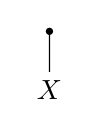
\begin{tikzpicture}[scale=0.75]
  \filldraw
    (0,0) node[fill=white] {$X$}
    --
    (0,1) circle (1.5pt) node[below right] {};
\end{tikzpicture}
\]
We want to be able to compose operations if one output matches an input of the other. For example, if we take
\begin{align*}
  f
  \in
  O(X_{1},X_{2},X_{3},X)
  \\
  f_{1}
  \in
  O(X_{11},X_{12},X_{1})
  \\
  f_{2}
  \in
  O(\emptyset,X)
  \\
  f_{3}
  \in
  O(X_{31},X_{3})
\end{align*}
then we want the composition illustrated by
\[
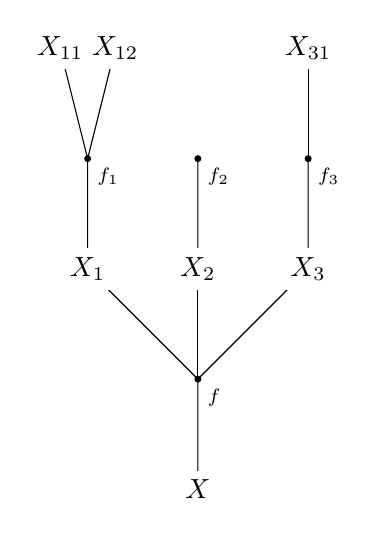
\begin{tikzpicture}[scale=0.70]
  \filldraw
    (0,0) node[fill=white] {$X$}
    --
    (0,2) circle (1.5pt) node[below right] {\scriptsize{$f$}};
  \draw
    (0,2)
    --
    (-2,4) node[fill=white] {$X_{1}$};
  \draw
    (0,2)
    --
    (0,4) node[fill=white] {$X_{2}$};
  \draw
    (0,2)
    --
    (2,4) node[fill=white] {$X_{3}$};
  \filldraw
    (-2,4) node[fill=white] {$X_{1}$}
    --
    (-2,6)
    circle (1.5pt) node[below right] {\scriptsize{$f_{1}$}};
  \draw
    (-2,6)
    --
    (-2.5,8) node[fill=white] {$X_{11}$};
  \draw
    (-2,6)
    --
    (-1.5,8) node[fill=white] {$X_{12}$};
  \filldraw
    (0,4) node[fill=white] {$X_{2}$}
    --
    (0,6) circle (1.5pt) node[below right] {\scriptsize{$f_{2}$}};
  \filldraw
    (2,4) node[fill=white] {$X_{3}$}
    --
    (2,6) circle (1.5pt) node[below right] {\scriptsize{$f_{3}$}};
  \draw
    (2,6)
    --
    (2,8) node[fill=white] {$X_{31}$};
\end{tikzpicture}
\]
to exist such that this composition is associative and in each set $O(X_{1},X_{2})$ with $X_{1},X_{2}$ arbitrary there is an element for each arrow from $X_{1}$ to $X_{2}$ in $\mathbf{C}$ behaving like an identity for identity arrows under the operad composition. Moreover one demands the composition to be {\glqq}stable{\grqq} under permutations of the input. What all this means precisely has to be looked up in a source about operads such as \cite{0d7b89ad}. It shall be not very surprising that operads abstractly track composition and hence that they have applications in higher category theory. Indeed, they are the backbone of a serious attempt to define weak $n$-category by Baez and Dolan in \cite{0d7b89ad}. It is not used much any more due to the addressed problems of weak $n$-categories for finite $n$ but it is a landmark paper in higher category theory and provides much intuition about the idea of higher category theory (and also operads). However, you might wish to first read \cite{de09a3f9} followed by \cite{c2d89e8a} which escort you more or less softly into the realms of higher category theory. In general, all the Baez stuff is highly recommended.
